\documentclass[border=10mm]{standalone}
\usepackage{tikz}
\usetikzlibrary{arrows, shapes.gates.logic.US, shapes.gates.logic.IEC, calc}

\tikzset{
    my-not-gate/.style={
        not gate US, draw, rotate=0, logic gate inputs=nn
    },
}

\begin{document}

\resizebox{10cm}{!}{

    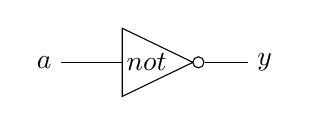
\begin{tikzpicture}[label distance=2mm]

        % INPUTS
        \node[] (A)    at (0,0)  {\normalsize $a$};

        % OUTPUTS
        \node[] (Y)    at (2.8,0)  {\normalsize $y$};
        
        % NOT, WIRES NOT CONNECTOR POINTS
        \node[my-not-gate]  (NOT)    at ($(A) + (1.3, 0)$)         {\normalsize $not$};
        \coordinate[]       (NOTIN1) at ($(NOT.input)   + (-.5, 0)$) {};
        \coordinate[]       (NOTOUT) at ($(NOT.output)  + (.5, 0)$)  {};
        \draw (NOT.input) --   (NOTIN1);
        \draw (NOT.output)  -- (NOTOUT);

        % INPUT CONNECTIONS
        \draw (A) -- (NOTIN1);
        
        % OUTPUT CONNECTIONS
        \draw (NOTOUT) -- (Y);

    \end{tikzpicture}
}

\end{document} 
